%==============================================================================
%  PROJECT REPORT  —  Offline Multi-Agent RAG-Based Virtual Assistant
%  Compile with:  pdflatex report.tex   (run twice for the ToC/refs)
%  Easiest: paste into a blank Overleaf project and click "Recompile".
%  Self-contained: standard packages only, no external image files required.
%==============================================================================
\documentclass[12pt,a4paper]{report}

%------------------------- packages ------------------------------------------
\usepackage[utf8]{inputenc}
\usepackage[T1]{fontenc}
\usepackage{lmodern}
\usepackage[a4paper,left=1.4in,right=1in,top=1in,bottom=1in]{geometry}
\usepackage{setspace}
\usepackage{graphicx}
\usepackage{booktabs}
\usepackage{array}
\usepackage{longtable}
\usepackage{amsmath}
\usepackage{amssymb}
\usepackage{xcolor}
\usepackage{listings}
\usepackage{caption}
\usepackage{titlesec}
\usepackage{fancyhdr}
\usepackage{enumitem}
\usepackage{tikz}
\usetikzlibrary{shapes.geometric,arrows.meta,positioning,calc,fit,backgrounds}
\usepackage[hidelinks]{hyperref}

%------------------------- editable metadata ---------------------------------
% >>> CHANGE THESE FIVE LINES <<<
\newcommand{\ProjectTitle}{Offline Multi-Agent RAG-Based Virtual Assistant}
\newcommand{\StudentName}{[Your Name]}
\newcommand{\StudentID}{[Your USN / Roll No.]}
\newcommand{\GuideName}{[Guide Name \& Designation]}
\newcommand{\InstituteName}{[Your College / University Name]}
\newcommand{\DeptName}{Department of Computer Science and Engineering}
\newcommand{\AcademicYear}{2025--2026}

%------------------------- style ---------------------------------------------
\onehalfspacing
\setlength{\parindent}{0pt}
\setlength{\parskip}{6pt}

\definecolor{codebg}{RGB}{247,247,249}
\definecolor{codekw}{RGB}{0,84,159}
\definecolor{codecm}{RGB}{110,110,110}
\lstset{
  backgroundcolor=\color{codebg},
  basicstyle=\ttfamily\footnotesize,
  keywordstyle=\color{codekw}\bfseries,
  commentstyle=\color{codecm}\itshape,
  breaklines=true,
  frame=single,
  rulecolor=\color{gray!40},
  showstringspaces=false,
  columns=fullflexible,
  captionpos=b,
}

\titleformat{\chapter}[display]
  {\normalfont\huge\bfseries}{\chaptertitlename\ \thechapter}{16pt}{\Large}
\titlespacing*{\chapter}{0pt}{-20pt}{24pt}

\pagestyle{fancy}
\fancyhf{}
\fancyhead[L]{\small Offline Multi-Agent RAG-Based Virtual Assistant}
\fancyhead[R]{\small\thepage}
\renewcommand{\headrulewidth}{0.4pt}

%==============================================================================
\begin{document}

%------------------------- TITLE PAGE ----------------------------------------
\begin{titlepage}
\centering
\vspace*{0.4in}
{\large A Project Report on\par}
\vspace{0.3in}
{\LARGE\bfseries \ProjectTitle \par}
\vspace{0.4in}
{\large \textit{Submitted in partial fulfillment of the requirements for the award of the degree of}\par}
\vspace{0.15in}
{\large\bfseries Bachelor of Engineering\par}
{\large in\par}
{\large\bfseries Computer Science and Engineering\par}
\vspace{0.4in}
{\large \textit{Submitted by}\par}
\vspace{0.1in}
{\large\bfseries \StudentName\par}
{\large \StudentID\par}
\vspace{0.4in}
{\large \textit{Under the guidance of}\par}
{\large\bfseries \GuideName\par}
\vfill
% --- Optional: place your college logo file here and uncomment:
% \includegraphics[width=0.25\textwidth]{logo.png}\par\vspace{0.2in}
{\large\bfseries \DeptName\par}
{\large\bfseries \InstituteName\par}
\vspace{0.15in}
{\large \AcademicYear\par}
\end{titlepage}

%------------------------- front matter --------------------------------------
\pagenumbering{roman}

% ---------------- ACKNOWLEDGEMENT ----------------
\chapter*{Acknowledgement}
\addcontentsline{toc}{chapter}{Acknowledgement}
I would like to express my sincere gratitude to everyone who supported me
throughout the course of this project.

I am deeply thankful to my guide, \GuideName, for the continuous guidance,
encouragement, and valuable feedback that shaped this work. I extend my thanks
to the \DeptName, \InstituteName, for providing the resources and environment
necessary to carry out this project.

I am also grateful to the open-source community whose tools and pre-trained
models---Docling, the BGE embedding and reranker family, Ollama, and the
Llama and Qwen model families---made this system possible. Finally, I thank my
family and friends for their constant support and motivation.

\vspace{0.5in}
\hfill \StudentName \\
\hfill \StudentID

% ---------------- ABSTRACT ----------------
\chapter*{Abstract}
\addcontentsline{toc}{chapter}{Abstract}
Large Language Models (LLMs) generate fluent text but are prone to
\emph{hallucination}---producing confident answers that are not grounded in any
real source---and typically require uploading private documents to third-party
cloud APIs. This project presents an \textbf{Offline Multi-Agent RAG-Based
Virtual Assistant}: a fully offline, multimodal question-answering assistant that
answers natural-language questions over the user's own PDF documents while running
entirely on a \textbf{modest 4~GB consumer laptop GPU (NVIDIA RTX~3050)}.

The assistant is built on a \textbf{multi-agent architecture} in which specialised
agents cooperate to answer a query: a \emph{Router Agent} classifies the query's
intent, a \emph{Text Agent} retrieves and reranks evidence, a \emph{Generator
Agent} produces a grounded answer with the local LLM, and an \emph{Image Agent}
surfaces figures for a vision-language model to interpret. This separation of
concerns keeps each stage focused, testable, and independently upgradeable.

Documents are ingested with \textbf{Docling}, which performs layout analysis,
table-structure recovery (TableFormer), and OCR (RapidOCR) so that both digital
and scanned PDFs---including tables and figures---are captured. Content is divided
using \textbf{semantic chunking}, enriched with a deterministic heading-path
context, and embedded with \texttt{BAAI/bge-base-en-v1.5}. At query time the Text
Agent runs a \textbf{hybrid retriever} that combines dense vector search with
sparse BM25 scoring, fused via Reciprocal Rank Fusion (RRF), followed by a
\textbf{cross-encoder reranker} (\texttt{bge-reranker-v2-m3}). A \textbf{multi-signal
grounding gate} decides whether the evidence is strong enough to answer or whether
to refuse safely, minimising hallucination. Grounded context is answered by
\texttt{llama3.2:3b}; figures are interpreted by \texttt{qwen2.5vl:3b}.

Evaluated on a 30-question benchmark derived from a domain FAQ, the assistant
produced substantively correct answers for approximately \textbf{70\%} of
questions while correctly refusing when evidence was insufficient. This
demonstrates that a carefully engineered multi-agent retrieval pipeline can
deliver reliable, private, grounded document question answering even under tight
hardware constraints. The report also analyses the accuracy ceiling imposed by
3-billion-parameter models on 4~GB hardware and outlines the changes required to
scale the same architecture to larger GPUs.

\tableofcontents
\listoffigures
\listoftables

%==============================================================================
\clearpage
\pagenumbering{arabic}

%==============================================================================
\chapter{Introduction}

\section{Introduction}
The volume of information stored in unstructured documents---technical manuals,
handbooks, standards, lecture notes, and reports---continues to grow rapidly.
Locating a specific fact inside a large PDF is slow and tedious with traditional
keyword search, which matches words but not meaning. Large Language Models (LLMs)
can read and summarise text fluently, but on their own they suffer from two
serious problems. First, they \emph{hallucinate}: when they do not know an answer
they often invent one that sounds plausible. Second, using a hosted LLM API
requires uploading potentially confidential documents to an external server.

\textbf{Retrieval-Augmented Generation (RAG)} tackles the first problem by
retrieving relevant passages from a trusted document collection and instructing
the LLM to answer \emph{only} from those passages, with the source available for
verification. Running the entire pipeline \emph{locally} tackles the second: no
document or query ever leaves the user's machine.

This project realises these ideas as an \textbf{Offline Multi-Agent RAG-Based
Virtual Assistant}. Rather than a single monolithic program, the assistant is
organised as a set of cooperating \emph{agents}---each responsible for one part of
answering a question (routing, retrieval, generation, and figure understanding).
This multi-agent design mirrors how a competent human assistant would work:
first understand what is being asked, then find the relevant evidence, then answer
strictly from that evidence, and consult a diagram when the question is visual.
The assistant is also \textbf{multimodal}---it understands paragraphs, tables, and
figures---and \textbf{resource-aware}, designed to run end to end on a 4~GB laptop
GPU rather than a data-centre accelerator. The result is a private, grounded, and
practical document question-answering assistant.

\section{Company Profile}
% >>> Replace the paragraph below with your organisation / college profile. <<<
This project was carried out at \InstituteName{} under the \DeptName.
\textit{[If this was an internship, replace this section with the profile of the
host company: its name, domain, products/services, and the team in which the
project was executed. If it was an in-house academic project, briefly describe
the department, its focus areas, and the laboratory facilities used.]}

\section{Problem Statement}
Organisations and individuals possess large collections of PDF documents but lack
a fast, trustworthy way to ask questions of them. Existing approaches fall short:

\begin{itemize}[leftmargin=1.4em]
  \item \textbf{Keyword search} returns pages, not answers, and misses
        semantically related wording.
  \item \textbf{General-purpose LLMs} hallucinate and cannot cite a source,
        making their answers unsafe for factual or numeric queries.
  \item \textbf{Cloud RAG services} require uploading private documents and incur
        recurring cost and network dependence.
  \item \textbf{Most open RAG demos} handle only clean digital text and ignore
        tables, scanned pages, and figures---exactly where technical answers live.
\end{itemize}

\textbf{The problem:} design a virtual assistant that answers natural-language
questions over a user's own PDFs \emph{accurately, with a verifiable source,
entirely offline, and on modest consumer hardware}, while correctly handling
tables and figures and refusing to answer when the documents do not contain the
information.

\section{Objectives of the Project}
\begin{enumerate}[leftmargin=1.6em]
  \item To design a \textbf{multi-agent architecture} in which specialised agents
        (routing, retrieval, generation, and image handling) cooperate to answer a
        query, giving a modular and maintainable system.
  \item To ingest both digital and scanned PDFs, preserving layout, tables, and
        figures, using a layout-aware document parser.
  \item To design a chunking and indexing strategy that keeps semantically
        coherent passages together and generalises to arbitrary documents.
  \item To implement a hybrid retrieval pipeline combining dense semantic search,
        sparse lexical search, and cross-encoder reranking for high precision.
  \item To ground every answer in retrieved evidence and to \emph{refuse safely}
        when evidence is insufficient, minimising hallucination.
  \item To interpret figures and diagrams using a vision-language model.
  \item To run the complete assistant offline on a 4~GB consumer GPU and expose it
        through a web interface.
  \item To evaluate answer quality on a question--answer benchmark and to
        characterise the system's accuracy limits.
\end{enumerate}

\section{Scope of the Project}
\textbf{In scope:} local ingestion of PDF documents; text, table, and figure
understanding; a multi-agent query pipeline with hybrid retrieval and reranking;
grounded answer generation with a local LLM and a vision-language model; a
browser-based user interface; and quantitative evaluation on a benchmark of
questions.

\textbf{Out of scope:} fine-tuning or training new foundation models from scratch;
multi-user cloud deployment and authentication; support for non-PDF formats such
as audio or video; and real-time collaborative editing. These are noted as
possible future extensions in Chapter~6.

%==============================================================================
\chapter{Literature Review}

Retrieval-Augmented Generation was introduced by Lewis et al.~\cite{ref:rag},
who combined a neural retriever with a sequence-to-sequence generator so that a
model could ground its output in an external, updatable knowledge source. This
framework directly reduces hallucination and lets the knowledge base change
without retraining the model.

\textbf{Dense retrieval.} Karpukhin et al.~\cite{ref:dpr} showed that
dual-encoder ``dense passage retrieval'' outperforms traditional term matching by
embedding queries and passages into a shared vector space. The quality of these
embeddings is decisive; the BGE (BAAI General Embedding) family~\cite{ref:bge}
and the multilingual BGE-M3 model~\cite{ref:bgem3} are among the strongest openly
available text encoders, and the reranker variant provides a cross-encoder for
high-precision re-scoring. Sentence-Transformers~\cite{ref:sbert} provides the
practical framework for computing and comparing such embeddings.

\textbf{Sparse retrieval and fusion.} Classical lexical ranking with
BM25~\cite{ref:bm25} remains a strong baseline, particularly for rare terms,
codes, and exact numbers that dense encoders may smooth over. Combining a dense
and a sparse ranking is most robustly done with Reciprocal Rank Fusion
(RRF)~\cite{ref:rrf}, which merges ranked lists without needing to calibrate
score scales.

\textbf{Chunking and context.} How a document is split strongly affects
retrieval. Fixed-size splitting can cut sentences mid-thought, whereas
\emph{semantic chunking} places boundaries where the topic actually shifts.
The ``small-to-big'' or parent-document pattern popularised by
LlamaIndex~\cite{ref:llamaindex} embeds small, precise child passages for
matching but returns their larger parent passage for answering. Anthropic's
\emph{Contextual Retrieval}~\cite{ref:contextual} demonstrated that prepending a
short description of where a chunk sits in its document markedly improves
retrieval accuracy.

\textbf{Document understanding.} Extracting clean structure from PDFs---
especially tables and scanned pages---is a hard problem. Docling~\cite{ref:docling}
provides an integrated pipeline of layout analysis, the TableFormer
table-structure model, and OCR, producing a structured representation suitable
for downstream RAG.

\textbf{Agent-based LLM systems.} A growing body of work organises LLM
applications as multiple cooperating \emph{agents}, each with a focused role,
rather than a single prompt. Decomposing a task across specialised components
improves modularity, controllability, and reliability~\cite{ref:react}. This
project applies the same principle at the system level: distinct routing,
retrieval, generation, and vision agents.

\textbf{Local generation and multimodality.} The availability of capable
open-weight models that run locally---Meta's Llama~3.2~\cite{ref:llama} for text
and Alibaba's Qwen2.5-VL~\cite{ref:qwenvl} for vision-language understanding---
served through runtimes such as Ollama~\cite{ref:ollama}, makes fully offline,
multimodal RAG feasible on consumer hardware. Vector storage and similarity search
in this project are handled by ChromaDB~\cite{ref:chroma}.

\textbf{Summary of the gap.} While each component is well studied individually,
most published demonstrations assume clean digital text and abundant GPU memory.
This project integrates layout-aware multimodal ingestion, semantic and contextual
chunking, hybrid retrieval with reranking, a safety-oriented grounding gate, and a
multi-agent query pipeline into a single assistant that runs within a 4~GB VRAM
budget.

%==============================================================================
\chapter{System Analysis and Design}

\section{Requirement Analysis}
\subsection{Functional Requirements}
\begin{itemize}[leftmargin=1.4em]
  \item Upload and ingest one or more PDF documents.
  \item Extract text, tables, and figures, including from scanned pages.
  \item Accept a natural-language question and return a grounded answer with its
        source passage.
  \item Interpret a figure referenced by a question using a vision model.
  \item Refuse to answer when the documents do not contain the information.
  \item Present all of the above through a web browser.
\end{itemize}

\subsection{Non-Functional Requirements}
\begin{itemize}[leftmargin=1.4em]
  \item \textbf{Privacy:} operate fully offline; no data leaves the machine.
  \item \textbf{Resource efficiency:} run on a 4~GB VRAM consumer GPU.
  \item \textbf{Accuracy \& safety:} maximise grounded correctness and minimise
        hallucination.
  \item \textbf{Modularity:} organise the query pipeline as independent agents.
  \item \textbf{Generality:} work on arbitrary PDFs, not one specific document.
  \item \textbf{Responsiveness:} stream answers token-by-token to the UI.
\end{itemize}

\section{System Architecture}
The system is organised as a two-phase pipeline: an offline \emph{ingestion} phase
that indexes documents, and an online \emph{query} phase in which a team of agents
answers questions. Figure~\ref{fig:arch} shows the end-to-end flow.

\begin{figure}[htbp]
\centering
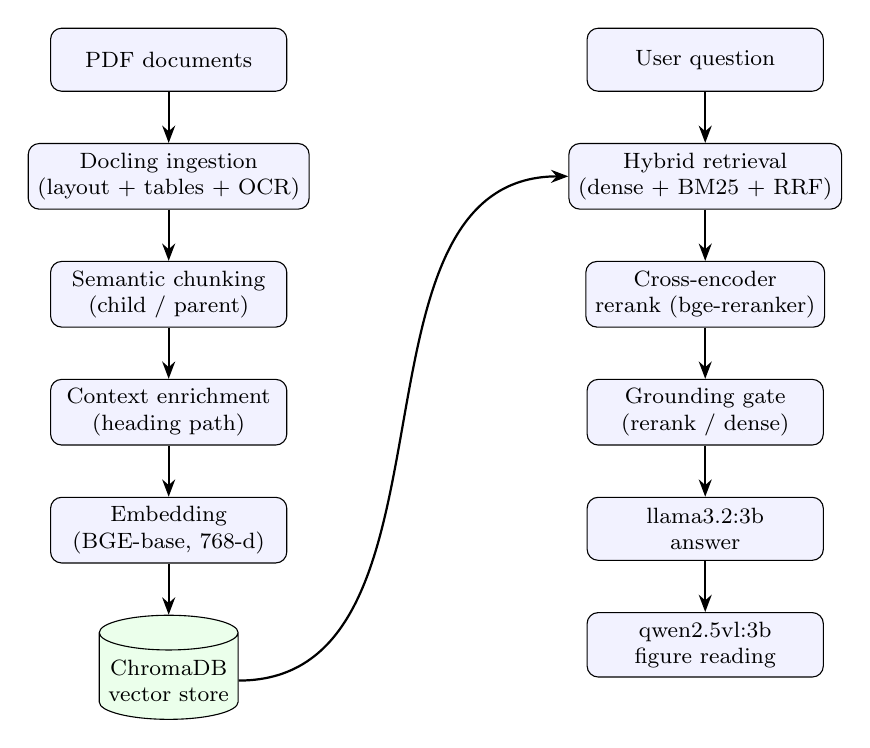
\begin{tikzpicture}[
  node distance=6.5mm and 10mm,
  box/.style={draw, rounded corners, align=center, font=\footnotesize,
              minimum height=8mm, minimum width=30mm, fill=blue!5},
  db/.style={draw, cylinder, shape border rotate=90, aspect=0.25,
             align=center, font=\footnotesize, fill=green!8, minimum height=12mm},
  arr/.style={-{Stealth[length=2.2mm]}, thick}
]
% ingestion column
\node[box] (pdf)   {PDF documents};
\node[box, below=of pdf]  (dl)   {Docling ingestion\\(layout + tables + OCR)};
\node[box, below=of dl]   (chunk){Semantic chunking\\(child / parent)};
\node[box, below=of chunk](ctx)  {Context enrichment\\(heading path)};
\node[box, below=of ctx]  (emb)  {Embedding\\(BGE-base, 768-d)};
\node[db,  below=of emb]  (store){ChromaDB\\vector store};
\draw[arr] (pdf)--(dl); \draw[arr] (dl)--(chunk); \draw[arr] (chunk)--(ctx);
\draw[arr] (ctx)--(emb); \draw[arr] (emb)--(store);

% query column
\node[box, right=38mm of pdf] (q)     {User question};
\node[box, below=of q]        (hyb)   {Hybrid retrieval\\(dense + BM25 + RRF)};
\node[box, below=of hyb]      (rr)    {Cross-encoder\\rerank (bge-reranker)};
\node[box, below=of rr]       (gate)  {Grounding gate\\(rerank / dense)};
\node[box, below=of gate]     (gen)   {llama3.2:3b\\answer};
\node[box, below=of gen]      (vlm)   {qwen2.5vl:3b\\figure reading};
\draw[arr] (q)--(hyb); \draw[arr] (hyb)--(rr); \draw[arr] (rr)--(gate);
\draw[arr] (gate)--(gen); \draw[arr] (gen)--(vlm);
\draw[arr] (store.east) to[out=0,in=180] (hyb.west);
\end{tikzpicture}
\caption{End-to-end architecture: offline ingestion (left) builds the vector
index; the online query phase (right) retrieves, reranks, gates, and generates.}
\label{fig:arch}
\end{figure}

\section{Multi-Agent Architecture}
The heart of the assistant is a set of four cooperating agents, each with a single
responsibility. Splitting the query pipeline this way makes every stage small,
independently testable, and upgradeable without touching the others.
Table~\ref{tab:agents} lists the agents and Figure~\ref{fig:agents} shows how they
interact.

\begin{table}[htbp]
\centering
\caption{The four agents and their responsibilities.}
\label{tab:agents}
\begin{tabular}{@{}p{3.0cm}p{3.0cm}p{6.6cm}@{}}
\toprule
\textbf{Agent} & \textbf{Module} & \textbf{Responsibility} \\
\midrule
Router Agent    & \texttt{router.py}          & Classify query intent---text answer vs.\ visual (figure) request---using fast rule-based keyword routing, avoiding an extra LLM round-trip. \\
Text Agent      & \texttt{text\_agent.py}     & Retrieve and rerank evidence: encode query (BGE) $\rightarrow$ ChromaDB top-20 $\rightarrow$ cross-encoder rerank $\rightarrow$ top-5, then apply the multi-signal grounding gate. \\
Generator Agent & \texttt{generator\_agent.py}& Build the grounded prompt, call the local LLM (\texttt{llama3.2:3b}), stream the answer, and refuse when no grounded evidence survives the gate. \\
Image Agent     & \texttt{image\_agent.py}    & Surface the figure(s) attached to the top chunks (de-duplicated, capped), which are then interpreted by the vision model \texttt{qwen2.5vl:3b}. \\
\bottomrule
\end{tabular}
\end{table}

\begin{figure}[htbp]
\centering
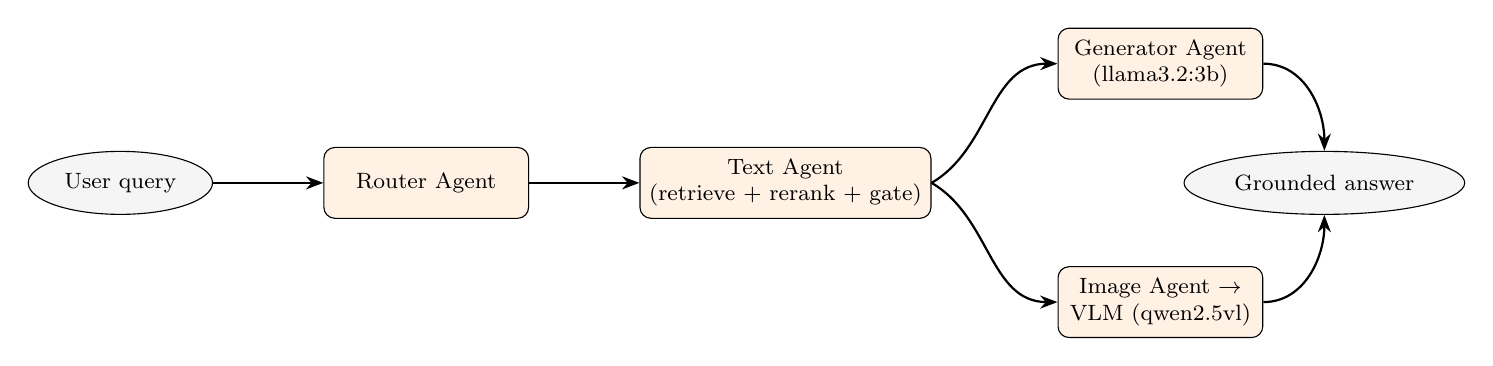
\begin{tikzpicture}[
  node distance=9mm and 14mm,
  ag/.style={draw, rounded corners, align=center, font=\footnotesize,
             minimum height=9mm, minimum width=26mm, fill=orange!10},
  io/.style={draw, ellipse, align=center, font=\footnotesize, fill=gray!8,
             minimum height=8mm},
  arr/.style={-{Stealth[length=2.2mm]}, thick}
]
\node[io] (q) {User query};
\node[ag, right=of q] (router) {Router Agent};
\node[ag, right=of router] (text) {Text Agent\\(retrieve + rerank + gate)};
\node[ag, above right=6mm and 16mm of text] (gen) {Generator Agent\\(llama3.2:3b)};
\node[ag, below right=6mm and 16mm of text] (img) {Image Agent $\rightarrow$\\VLM (qwen2.5vl)};
\node[io, right=32mm of text] (ans) {Grounded answer};
\draw[arr] (q)--(router);
\draw[arr] (router)--(text);
\draw[arr] (text.east) to[out=30,in=180] (gen.west);
\draw[arr] (text.east) to[out=-30,in=180] (img.west);
\draw[arr] (gen.east) to[out=0,in=90] (ans.north);
\draw[arr] (img.east) to[out=0,in=-90] (ans.south);
\end{tikzpicture}
\caption{Multi-agent interaction: the Router Agent classifies intent; the Text
Agent gathers grounded evidence; the Generator Agent produces the text answer and
the Image Agent routes figures to the vision model.}
\label{fig:agents}
\end{figure}

\section{Technology Stack}
Table~\ref{tab:stack} lists the main technologies and the role each plays.

\begin{table}[htbp]
\centering
\caption{Technology stack.}
\label{tab:stack}
\begin{tabular}{@{}p{3.4cm}p{3.2cm}p{6.2cm}@{}}
\toprule
\textbf{Layer} & \textbf{Technology} & \textbf{Role} \\
\midrule
Ingestion      & Docling 2.111            & Layout analysis, TableFormer, RapidOCR \\
Embeddings     & bge-base-en-v1.5         & 768-dim dense text encoder \\
Reranker       & bge-reranker-v2-m3       & Cross-encoder candidate re-scoring \\
Sparse search  & rank-bm25                & Lexical / exact-term retrieval \\
Vector store   & ChromaDB                 & Similarity search over embeddings \\
Text LLM       & llama3.2:3b (Ollama)     & Grounded answer generation \\
Vision model   & qwen2.5vl:3b (Ollama)    & Figure and diagram interpretation \\
Backend        & FastAPI + Uvicorn        & REST / streaming API \\
Frontend       & React + Vite             & Browser user interface \\
Runtime        & Python 3.11, PyTorch (CUDA 12.6) & Model execution \\
\bottomrule
\end{tabular}
\end{table}

\section{Hardware and Software Environment}
The system was developed and evaluated on an NVIDIA RTX~3050 Laptop GPU with 4~GB
of VRAM, using CUDA~12.6 and PyTorch~2.12.1. Embedding and reranking run on the
GPU or CPU depending on available memory, and the two Ollama models are loaded one
at a time to fit within the VRAM budget. All models are stored locally so the
system requires no network access after setup.

%==============================================================================
\chapter{Methodology and Implementation}

This chapter describes the assistant stage by stage, following a document from a
raw PDF to a grounded answer, and then explains how the four agents orchestrate the
query phase.

\section{Document Ingestion with Docling}
Each PDF is processed by Docling, which runs three cooperating models: a
\emph{layout} model that identifies the reading order and the type of each region
(heading, paragraph, table, figure); the \emph{TableFormer} model that recovers
the row/column structure of tables; and \emph{RapidOCR}, which reads text from
scanned or image-only pages. Digital PDFs are parsed directly, while scanned pages
fall back to OCR automatically. The output is a structured list of elements---each
with a type, page number, bounding box, section, heading, and content---plus
cropped images of every figure for later visual interpretation.

\section{Semantic Chunking}
Retrieval quality depends heavily on how documents are divided. Rather than
splitting on a fixed character count, the system uses \textbf{semantic chunking}:
consecutive sentences are embedded and the boundary between two chunks is placed
where the semantic distance between neighbouring sentences is largest (above a
percentile threshold), so that each chunk stays on a single topic. Tables are
handled specially and split at the row level so that a query can match an
individual row of data.

A \textbf{small-to-big (parent--child)} scheme is used. Each chunk is stored with
a short, precise \emph{child} passage (used for embedding and matching) and a
larger \emph{parent} passage (returned to the LLM for answering). This gives the
retriever pinpoint matching while giving the generator enough surrounding context.

\begin{table}[htbp]
\centering
\caption{Key chunking parameters.}
\label{tab:chunk}
\begin{tabular}{@{}lp{8.5cm}@{}}
\toprule
\textbf{Parameter} & \textbf{Purpose / value} \\
\midrule
Target chunk length     & $\approx$1000 characters (parent) \\
Maximum chunk length    & 1800 characters \\
Child split length      & $\approx$450 characters (embedded unit) \\
Minimum chunk length    & 60 characters (merge shorter fragments) \\
Split percentile        & 90th percentile of sentence-distance \\
Table handling          & row-level chunks, capped per table \\
\bottomrule
\end{tabular}
\end{table}

\section{Context Enrichment}
Before embedding, each child passage is prefixed with a deterministic
\textbf{context string} built from its position in the document---the document
title, section, and heading path (for example, ``\texttt{FCC Handbook --
Catalyst > Regeneration}''). This inexpensive, LLM-free step follows the idea of
Contextual Retrieval~\cite{ref:contextual}: it disambiguates otherwise generic
passages and measurably improves retrieval, without the cost of calling an LLM on
every chunk at ingestion time.

\section{Embedding and Vector Storage}
The context-enriched child passages are encoded with
\texttt{BAAI/bge-base-en-v1.5} into 768-dimensional vectors and stored in ChromaDB
together with their metadata and parent text. ChromaDB uses an L2 index; cosine
similarity is recovered as $\text{cos} = 1 - d/2$, which is later used as one of
the grounding signals.

\section{The Query Pipeline: Agents in Action}
When the user asks a question, the four agents run in sequence.

\subsection{Router Agent}
The Router Agent first classifies the query's intent. Using a fast rule-based
check for visual keywords (``figure'', ``diagram'', ``show'', \dots), it decides
whether the user wants a text answer or a visual, so that the pipeline can involve
the Image Agent only when needed. Rule-based routing avoids an extra LLM call, so
answers begin streaming sooner.

\subsection{Text Agent --- Hybrid Retrieval}
The Text Agent runs two retrievers in parallel:
\begin{itemize}[leftmargin=1.4em]
  \item a \textbf{dense} search that embeds the query and finds the nearest
        vectors (semantic matches), and
  \item a \textbf{sparse} BM25 search over the same context-enriched text
        (exact-term and numeric matches).
\end{itemize}
The two ranked lists are merged with \textbf{Reciprocal Rank Fusion}:
\begin{equation}
\text{RRF}(d) = \sum_{r \in \{\text{dense},\,\text{sparse}\}} \frac{1}{k + \text{rank}_r(d)}, \qquad k = 60 .
\end{equation}
RRF rewards documents that rank highly in \emph{either} retriever without needing
to normalise their different score scales. The query is also spelling-normalised
against the corpus vocabulary to tolerate typos. Roughly the top~20 fused
candidates are passed on, and matched child passages are expanded to their parent
passages so the generator sees full context.

\subsection{Text Agent --- Cross-Encoder Reranking}
The fused candidates are re-scored by the \texttt{bge-reranker-v2-m3}
cross-encoder, which reads the query and each candidate \emph{together} and is far
more precise than the bi-encoder used for first-stage retrieval. Two domain-aware
boosts are added: a \emph{heading/section overlap} boost, and a \emph{topic-gated
numeric} boost that rewards a candidate only when the query asks for a quantity
\emph{and} the candidate actually contains a number with a unit. The top~5
reranked passages are kept.

\subsection{Text Agent --- Multi-Signal Grounding Gate}
Before generating, the Text Agent decides whether the evidence is strong enough to
answer. A single threshold is brittle, so a \textbf{multi-signal gate} is used:
\begin{equation}
\text{answer} \iff (\text{rerank score} \ge 0.30) \;\lor\; (\text{max dense similarity} \ge 0.60).
\end{equation}
If neither signal is met, the assistant refuses with an honest ``the documents do
not contain enough information'' message rather than guessing. This is the primary
defence against hallucination. The two signals are complementary: the rerank score
is precise but its scale drifts across documents, while the dense cosine similarity
is corpus-stable and rescues awkwardly phrased in-scope questions.

\subsection{Generator Agent --- Answer Generation}
Passing the gate, the top passages are packed into the prompt up to a token budget
($\approx$1500 tokens) so as not to overflow the 3B model's context window;
because passages arrive best-first, only the least relevant are trimmed. The
Generator Agent instructs \texttt{llama3.2:3b} to answer strictly from the provided
context and streams the answer to the UI token by token. If no chunks survived the
gate, it returns the safe refusal message instead of calling the LLM.

\subsection{Image Agent --- Figure Interpretation}
When the Router Agent flags a visual query, or the retrieved evidence is a figure,
the Image Agent collects the cropped figure image(s) attached to the top chunks and
passes them to the \texttt{qwen2.5vl:3b} vision-language model, which describes or
interprets the diagram. To respect the 4~GB VRAM budget, the text model is evicted
before the vision model is loaded so that each has the full GPU in turn.

\section{API and User Interface}
A FastAPI backend exposes endpoints for ingestion, status, streaming query, and
figure interpretation, using Server-Sent Events to stream tokens. A React (Vite)
frontend lets the user upload PDFs, ask questions, watch answers stream in, and
view the cited source passage or figure.

\section{Offline Deployment}
All models---the embedder, the reranker, the Docling models, and the two Ollama
models---are downloaded once into a local folder by a helper script, after which
the assistant runs with no network access. A single \texttt{requirements.txt} and a
setup guide reproduce the environment on another machine.

%==============================================================================
\chapter{Results and Discussion}

\section{Evaluation Methodology}
The assistant was evaluated on a benchmark of \textbf{30 questions} derived from a
domain FAQ covering the ingested documents. Each generated answer was compared
against the reference answer and classified as \emph{Correct} (matches the
reference), \emph{Partially correct} (right topic, incomplete or imprecise),
\emph{Incorrect/Weak}, or \emph{Refused} (the system declined to answer).
An answer that is \emph{Correct} or \emph{Partially correct} is counted as
\emph{substantive}.

\section{Retrieval and Chunking Experiments}
Three chunking strategies were compared under the same retrieval and generation
settings. Semantic chunking gave the best balance of correct answers and safe
refusals, and was adopted as the final configuration
(Table~\ref{tab:chunkcompare}).

\begin{table}[htbp]
\centering
\caption{Effect of chunking strategy on answer quality (indicative counts).}
\label{tab:chunkcompare}
\begin{tabular}{@{}lccc@{}}
\toprule
\textbf{Strategy} & \textbf{Correct} & \textbf{Partial} & \textbf{Weak/Refused} \\
\midrule
Fixed coarse split   & 11 & 9 & 10 \\
Character split      & 10 & 8 & 12 \\
\textbf{Semantic (final)} & \textbf{13} & \textbf{8} & \textbf{9} \\
\bottomrule
\end{tabular}
\end{table}

\section{Overall Results}
With the final semantic-chunking configuration, the assistant produced substantive
answers for about \textbf{70\%} of the benchmark questions
(Table~\ref{tab:results}), while refusing safely on questions whose answers were
not present, rather than hallucinating.

\begin{table}[htbp]
\centering
\caption{Overall results on the 30-question benchmark.}
\label{tab:results}
\begin{tabular}{@{}lcc@{}}
\toprule
\textbf{Category} & \textbf{Count} & \textbf{Percentage} \\
\midrule
Correct                     & 13 & 43\% \\
Partially correct           & 8  & 27\% \\
Incorrect / Weak            & 7  & 23\% \\
Refused (safe)              & 2  & 7\%  \\
\midrule
\textbf{Substantive (Correct + Partial)} & \textbf{21} & \textbf{70\%} \\
\bottomrule
\end{tabular}
\end{table}

\section{Discussion}
Several patterns emerged from the error analysis:
\begin{itemize}[leftmargin=1.4em]
  \item \textbf{Text and definition questions} were answered most reliably; the
        hybrid retriever and reranker consistently surfaced the correct passage.
  \item \textbf{Exact-number and table questions} were the hardest. Failures had
        two causes: occasional retrieval misses, and---more often---the 3B
        generator paraphrasing or rounding a value that was present in the
        retrieved context. The topic-gated numeric boost in the reranker and
        row-level table chunking reduced but did not eliminate these errors.
  \item \textbf{The grounding gate behaved as intended}, refusing on out-of-scope
        questions instead of fabricating answers---the desired safety behaviour.
\end{itemize}

\subsection{The Hardware Ceiling}
Careful analysis showed that the remaining errors are dominated not by the
retrieval pipeline but by the \textbf{capacity of a 3-billion-parameter model on
4~GB of VRAM}. Multiple chunking and retrieval refinements all plateaued near the
same substantive-accuracy level, indicating that the bottleneck is generation, not
retrieval. On a larger GPU the identical multi-agent pipeline can host a 7B--14B
text model with a longer context window and GPU-accelerated encoders, which is
expected to raise exact-number accuracy substantially (an estimated
70\%~$\rightarrow$~85\%). The assistant was therefore engineered so that this
upgrade requires only changing the model name and a few capacity parameters, with
no change to the agents or pipeline.

%==============================================================================
\chapter{Conclusion and Future Scope}

\section{Conclusion}
This project delivered an \textbf{Offline Multi-Agent RAG-Based Virtual Assistant}
that answers natural-language questions over the user's own PDF documents on a
4~GB consumer GPU. By organising the query pipeline as four cooperating agents---
routing, retrieval, generation, and image handling---and combining layout-aware
ingestion, semantic and contextual chunking, hybrid dense--sparse retrieval with
cross-encoder reranking, a multi-signal grounding gate, and local text and vision
models, the assistant produces grounded, source-cited answers and refuses safely
when evidence is lacking. It achieved roughly 70\% substantive accuracy on a
30-question benchmark while preserving full privacy, meeting the objectives set out
in Chapter~1.

\section{Limitations}
\begin{itemize}[leftmargin=1.4em]
  \item \textbf{Model capacity:} the 3B text model limits precision on complex,
        multi-step, and exact-number questions.
  \item \textbf{VRAM budget:} only one model fits in memory at a time, so text and
        vision models must be swapped, adding latency to figure queries.
  \item \textbf{OCR on CPU:} scanned-document ingestion is slower because OCR runs
        on the CPU on the development hardware.
  \item \textbf{Single-user, local scope:} the assistant is not yet a multi-user
        service with authentication.
\end{itemize}

\section{Future Scope}
\begin{itemize}[leftmargin=1.4em]
  \item \textbf{Larger models on bigger GPUs:} switch the Generator Agent to a
        7B--14B model and enable GPU encoders and OCR for higher accuracy and speed.
  \item \textbf{More agents:} add a query-rewriting agent and a verification agent
        that checks an answer against its cited evidence before returning it.
  \item \textbf{Advanced retrieval:} add hierarchical summarisation (RAPTOR),
        proposition-level indexing, or late-interaction (ColBERT) reranking.
  \item \textbf{Broader inputs:} extend ingestion to office documents, HTML, and
        images beyond PDF.
  \item \textbf{Deployment:} package as a multi-user service with document-level
        access control and conversation memory.
\end{itemize}

\section{Overall Outcome}
The project demonstrates that reliable, private, grounded document question
answering is achievable on ordinary consumer hardware through careful engineering
rather than raw compute. The delivered assistant is modular, reproducible, and
directly scalable: the same multi-agent pipeline that runs on a 4~GB laptop today
will run with markedly higher accuracy on a larger GPU by changing only the model
configuration. Beyond the working software, the project produced a clear
understanding of where accuracy is won and lost in a RAG system---knowledge that
transfers to any future retrieval-augmented application.

%==============================================================================
\begin{thebibliography}{99}
\addcontentsline{toc}{chapter}{References}

\bibitem{ref:rag} P. Lewis et al., ``Retrieval-Augmented Generation for
Knowledge-Intensive NLP Tasks,'' \emph{NeurIPS}, 2020.

\bibitem{ref:dpr} V. Karpukhin et al., ``Dense Passage Retrieval for Open-Domain
Question Answering,'' \emph{EMNLP}, 2020.

\bibitem{ref:bge} S. Xiao et al., ``C-Pack: Packed Resources for General Chinese
Embeddings (BGE),'' \emph{arXiv:2309.07597}, 2023.

\bibitem{ref:bgem3} J. Chen et al., ``BGE M3-Embedding: Multi-Lingual,
Multi-Functionality, Multi-Granularity Text Embeddings,'' \emph{arXiv:2402.03216},
2024.

\bibitem{ref:sbert} N. Reimers and I. Gurevych, ``Sentence-BERT: Sentence
Embeddings using Siamese BERT-Networks,'' \emph{EMNLP}, 2019.

\bibitem{ref:bm25} S. Robertson and H. Zaragoza, ``The Probabilistic Relevance
Framework: BM25 and Beyond,'' \emph{Foundations and Trends in Information
Retrieval}, 2009.

\bibitem{ref:rrf} G. V. Cormack, C. L. A. Clarke, and S. Buettcher, ``Reciprocal
Rank Fusion Outperforms Condorcet and Individual Rank Learning Methods,''
\emph{SIGIR}, 2009.

\bibitem{ref:llamaindex} J. Liu, ``LlamaIndex: A Data Framework for LLM
Applications,'' 2023. [Online]. Available: \url{https://www.llamaindex.ai}

\bibitem{ref:contextual} Anthropic, ``Introducing Contextual Retrieval,'' 2024.
[Online]. Available: \url{https://www.anthropic.com/news/contextual-retrieval}

\bibitem{ref:docling} C. Auer et al., ``Docling Technical Report,'' IBM Research,
\emph{arXiv:2408.09869}, 2024.

\bibitem{ref:react} S. Yao et al., ``ReAct: Synergizing Reasoning and Acting in
Language Models,'' \emph{ICLR}, 2023.

\bibitem{ref:llama} Meta AI, ``Llama 3.2: Open Foundation Models,'' 2024.
[Online]. Available: \url{https://ai.meta.com/llama}

\bibitem{ref:qwenvl} Qwen Team, ``Qwen2.5-VL Technical Report,'' Alibaba, 2024.
[Online]. Available: \url{https://github.com/QwenLM/Qwen2.5-VL}

\bibitem{ref:ollama} Ollama, ``Run Large Language Models Locally,'' 2024.
[Online]. Available: \url{https://ollama.com}

\bibitem{ref:chroma} Chroma, ``ChromaDB: The AI-native Open-Source Embedding
Database,'' 2024. [Online]. Available: \url{https://www.trychroma.com}

\end{thebibliography}

\end{document}
